\documentclass[11pt]{article}

% Mandatory Packages
\usepackage{amsmath}
\usepackage{amssymb}
\usepackage{amsthm}
\usepackage{geometry}
\usepackage{tikz}
\usepackage{mathrsfs}
\usepackage{mathtools}
\usepackage{color}
\usepackage{enumitem}
\usepackage{booktabs}

% TikZ Libraries
\usetikzlibrary{arrows.meta, positioning, shapes, calc}

% Page Geometry
\geometry{letterpaper, margin=1in}

% Theorem Environments
\theoremstyle{definition}
\newtheorem{definition}{Definition}[section]
\theoremstyle{plain}
\newtheorem{theorem}{Theorem}[section]
\newtheorem{lemma}[theorem]{Lemma}
\newtheorem{proposition}[theorem]{Proposition}
\theoremstyle{remark}
\newtheorem{remark}{Remark}[section]

% Custom Commands for Math Sets and Probability
\newcommand{\R}{\mathbb{R}}
\newcommand{\N}{\mathbb{N}}
\newcommand{\F}{\mathcal{F}}
\newcommand{\B}{\mathcal{B}}
\newcommand{\E}{\mathbb{E}}
\renewcommand{\P}{\mathbb{P}}
\newcommand{\1}{\mathbf{1}}

\title{\textbf{Homework 2: Random Variables, Uniform Sampling, and Probability Spaces}}
\author{Tashfeen Omran}
\date{September 2026}

\begin{document}

\maketitle
\tableofcontents
\newpage

% ==========================================
% PART 1: INTRODUCTION AND PREREQUISITES
% ==========================================
\section{Comprehensive Introduction, Context, and Prerequisites}

\subsection{Historical Context and Motivation}
Historically, probability was treated as an informal extension of combinatorics, heavily tied to games of chance. However, as mathematicians attempted to analyze continuous phenomena and complex infinite sequences, the lack of a rigorous foundation led to severe paradoxes (such as Bertrand's Paradox). In 1933, Andrey Kolmogorov revolutionized the field by publishing \textit{Foundations of the Theory of Probability}. By synthesizing probability with the emerging fields of set theory and Lebesgue measure theory, Kolmogorov demonstrated that randomness could be completely formalized. This chapter transitions from elementary event-counting to this rigorous formulation, introducing the concept of a \textit{Random Variable} not merely as a variable that takes random values, but as a formal measurable mapping between algebraic spaces.

\subsection{Core Concepts, Axioms, and Definitions}
To rigorously evaluate probabilities and random samples, we must construct a mathematical framework known as a \textbf{Probability Space}, denoted by the triplet $(\Omega, \F, \P)$.

\begin{definition}[Sample Space $\Omega$]
The sample space $\Omega$ is an arbitrary, non-empty set containing all possible mutually exclusive outcomes of an experiment. An individual outcome is a sample point $\omega \in \Omega$.
\end{definition}

\begin{definition}[$\sigma$-Algebra $\F$]
A $\sigma$-algebra $\F$ is a collection of subsets of $\Omega$ that represents the set of all ``measurable'' events. It must satisfy three axioms:
\begin{enumerate}
    \item \textit{Non-emptiness:} $\Omega \in \F$.
    \item \textit{Closure under complementation:} If $A \in \F$, then $A^c \in \F$.
    \item \textit{Closure under countable union:} If $A_1, A_2, \dots \in \F$, then $\bigcup_{i=1}^\infty A_i \in \F$.
\end{enumerate}
\end{definition}

\begin{definition}[Probability Measure $\P$]
A probability measure $\P: \F \to [0, 1]$ is a set function satisfying Kolmogorov's Axioms:
\begin{enumerate}
    \item \textit{Non-negativity:} $\P(A) \ge 0$ for all $A \in \F$.
    \item \textit{Unitarity:} $\P(\Omega) = 1$.
    \item \textit{Countable Additivity:} For any countable sequence of pairwise disjoint sets $A_1, A_2, \dots \in \F$, $\P\left(\bigcup_{i=1}^\infty A_i\right) = \sum_{i=1}^\infty \P(A_i)$.
\end{enumerate}
\end{definition}

\begin{definition}[Random Variable]
A random variable $Y$ is a \textbf{measurable function} mapping the sample space to the real numbers, $Y: \Omega \to \R$. Measurability requires that for every Borel set $B \in \B(\R)$, the pre-image $Y^{-1}(B) = \{\omega \in \Omega \mid Y(\omega) \in B\}$ is an element of $\F$.
\end{definition}

\subsection{Key Theorems, Lemmas, and Formulas}
\begin{theorem}[Law of Total Probability (LOTP)]
Let $\{B_1, B_2, \dots, B_n\}$ be a finite partition of $\Omega$ such that $B_i \cap B_j = \emptyset$ for $i \neq j$ and $\bigcup_{i=1}^n B_i = \Omega$. If $\P(B_i) > 0$ for all $i$, then for any event $A \in \F$:
\[ \P(A) = \sum_{i=1}^n \P(A \mid B_i) \P(B_i) \]
\end{theorem}

\begin{theorem}[Bayes' Theorem]
Given a partition $\{B_1, \dots, B_n\}$ of $\Omega$, the conditional probability of $B_k$ given $A$ is:
\[ \P(B_k \mid A) = \frac{\P(A \mid B_k) \P(B_k)}{\sum_{i=1}^n \P(A \mid B_i) \P(B_i)} \]
\end{theorem}

\subsection{Prerequisites}
To fully comprehend this chapter, one must possess a mastery of:
\begin{itemize}
    \item \textbf{Set Theory:} Intersections ($\cap$), unions ($\cup$), complements ($^c$), and Cartesian products ($\times$).
    \item \textbf{Calculus \& Analysis:} Convergence of infinite geometric series, limit definitions.
    \item \textbf{Combinatorics:} Permutations, combinations ($\binom{n}{k}$), and the multiplication principle.
\end{itemize}

% ==========================================
% PART 2: DETAILED HOMEWORK SOLUTIONS
% ==========================================
\section{Detailed Homework Solutions (Rigorous Proofs \& Computations)}
Based on the provided PDF, a strategic selection of four distinct problem archetypes guarantees comprehensive mastery over the text's principles. 

\subsection{Problem 2.135: The Bayes' Partitioning Archetype}
\textbf{Problem Statement:} 
Of travelers arriving at a small airport, $60\%$ fly on major airlines, $30\%$ fly on privately owned planes, and the remainder fly on commercially owned planes not belonging to a major airline. Of those traveling on major airlines, $50\%$ are traveling for business, whereas $60\%$ of those on private planes and $90\%$ of those on other commercial planes are traveling for business. We select one arriving person at random. Find the probability that the person:
(a) is traveling on business?
(b) is traveling for business on a privately owned plane?
(c) arrived on a privately owned plane, given that the person is traveling for business?
(d) is traveling on business, given that the person is flying on a commercially owned plane?

\begin{proof}[Solution]
We establish a uniform probability space. Let the sample space $\Omega$ be the set of all travelers. We partition $\Omega$ into three mutually exclusive subsets based on flight type: $M$ (Major), $P$ (Private), and $C$ (Commercial). 
The prior probability measure $\P$ assigns:
\[ \P(M) = 0.60, \quad \P(P) = 0.30, \quad \P(C) = 1 - (0.60 + 0.30) = 0.10 \]
Let $B \in \F$ be the event ``traveling for business''. The conditional probabilities are provided as:
\[ \P(B \mid M) = 0.50, \quad \P(B \mid P) = 0.60, \quad \P(B \mid C) = 0.90 \]

\textbf{Part (a):} We apply the Law of Total Probability to find the marginal probability $\P(B)$.
\begin{align*}
\P(B) &= \P(B \mid M)\P(M) + \P(B \mid P)\P(P) + \P(B \mid C)\P(C) \\
      &= (0.50)(0.60) + (0.60)(0.30) + (0.90)(0.10) \\
      &= 0.30 + 0.18 + 0.09 = 0.57
\end{align*}

\textbf{Part (b):} We require the probability of the intersection $B \cap P$. Using the multiplication rule:
\begin{align*}
\P(B \cap P) &= \P(B \mid P) \P(P) \\
             &= (0.60)(0.30) = 0.18
\end{align*}

\textbf{Part (c):} We calculate the posterior probability $\P(P \mid B)$ using Bayes' Theorem.
\begin{align*}
\P(P \mid B) &= \frac{\P(B \cap P)}{\P(B)} \\
             &= \frac{0.18}{0.57} = \frac{18}{57} = \frac{6}{19} \approx 0.3158
\end{align*}

\textbf{Part (d):} We evaluate $\P(B \mid C)$. This is an explicit axiom given in the problem statement.
\[ \P(B \mid C) = 0.90 \]
\end{proof}
\textbf{Conclusion:} (a) $0.57$; (b) $0.18$; (c) $6/19$; (d) $0.90$. $\blacksquare$

\subsection{Problem 2.137: Combinatorial Sampling Without Replacement}
\textbf{Problem Statement:}
Five identical bowls are labeled $1, 2, 3, 4, 5$. Bowl $i$ contains $i$ white and $5 - i$ black balls. A bowl is randomly selected and two balls are selected (without replacement).
(a) What is the probability both balls are white?
(b) Given both are white, what is the probability bowl 3 was selected?

\begin{proof}[Solution]
Define the partition $\{B_1, B_2, B_3, B_4, B_5\}$ where $B_i$ is the event ``Bowl $i$ is chosen''.
Since sampling is uniform, $\P(B_i) = \frac{1}{5}$ for $i \in \{1, 2, 3, 4, 5\}$.
Let $W$ denote the event ``both drawn balls are white''.
Using hypergeometric combinatorics, the number of ways to draw $2$ white balls from $i$ available white balls, and $0$ black balls from $(5-i)$ available, out of a total of $\binom{5}{2}$ pairs is:
\[ \P(W \mid B_i) = \frac{\binom{i}{2}\binom{5-i}{0}}{\binom{5}{2}} = \frac{\frac{i(i-1)}{2}}{10} = \frac{i(i-1)}{20} \]
Evaluating this for each $i$:
\begin{align*}
\P(W \mid B_1) &= \frac{1(0)}{20} = 0 \\
\P(W \mid B_2) &= \frac{2(1)}{20} = \frac{2}{20} \\
\P(W \mid B_3) &= \frac{3(2)}{20} = \frac{6}{20} \\
\P(W \mid B_4) &= \frac{4(3)}{20} = \frac{12}{20} \\
\P(W \mid B_5) &= \frac{5(4)}{20} = \frac{20}{20} = 1
\end{align*}

\textbf{Part (a):} By the Law of Total Probability:
\begin{align*}
\P(W) &= \sum_{i=1}^5 \P(W \mid B_i)\P(B_i) \\
      &= \frac{1}{5} \left( 0 + \frac{2}{20} + \frac{6}{20} + \frac{12}{20} + \frac{20}{20} \right) \\
      &= \frac{1}{5} \left( \frac{40}{20} \right) = \frac{1}{5}(2) = \frac{2}{5} = 0.40
\end{align*}

\textbf{Part (b):} By Bayes' Theorem:
\begin{align*}
\P(B_3 \mid W) &= \frac{\P(W \mid B_3)\P(B_3)}{\P(W)} \\
               &= \frac{\left(\frac{6}{20}\right)\left(\frac{1}{5}\right)}{\frac{2}{5}} = \frac{\frac{6}{100}}{\frac{40}{100}} = \frac{6}{40} = 0.15
\end{align*}
\end{proof}
\textbf{Conclusion:} (a) $0.40$; (b) $0.15$. $\blacksquare$

\subsection{Problem 2.138: Infinite State Spaces \& Absorption (The Game of Craps)}
\textbf{Problem Statement:}
A player rolls two dice. If the first toss is 7 or 11, the player wins. If 2, 3, or 12, the player loses. Otherwise, the value becomes the ``point''. The player tosses the dice repeatedly until rolling the point (win) or a 7 (loss). Find the probability the player wins.

\begin{proof}[Solution]
Let $D_n \in \{2, \dots, 12\}$ be the random variable mapping the $n$-th toss of the two dice to their sum. 
The measure over the sample space of two dice yields $\P(D_n = k) = p_k$, where $p_7 = \frac{6}{36}$, $p_{11} = \frac{2}{36}$, $p_4 = p_{10} = \frac{3}{36}$, $p_5 = p_9 = \frac{4}{36}$, $p_6 = p_8 = \frac{5}{36}$.

Let $W$ be the event of winning the game. $W$ can occur on the first toss ($W_1$) or on a subsequent toss by matching a point $k$ ($W_k$).
\[ \P(W_1) = \P(D_1 = 7) + \P(D_1 = 11) = \frac{6}{36} + \frac{2}{36} = \frac{8}{36} = \frac{2}{9} \]

Suppose a point $k \in \{4, 5, 6, 8, 9, 10\}$ is established (event $E_k$). The conditional probability of winning, $\P(W \mid E_k)$, is the probability of the sequence of events where a $k$ is rolled before a $7$.
Let $A_{k,m}$ be the event that neither $k$ nor $7$ is rolled on tosses $2$ through $m$, and $k$ is rolled on toss $m+1$. Since tosses are independent, $\P(A_{k,m}) = (1 - p_k - p_7)^{m-1} p_k$. 
The total probability of rolling $k$ before $7$ is the countable union of mutually exclusive events:
\begin{align*}
\P(W \mid E_k) &= \sum_{m=1}^\infty (1 - p_k - p_7)^{m-1} p_k 
\end{align*}
This is an infinite geometric series with ratio $r = (1 - p_k - p_7)$. Since $0 \le r < 1$, it converges to $\frac{p_k}{1 - r}$:
\[ \P(W \mid E_k) = \frac{p_k}{1 - (1 - p_k - p_7)} = \frac{p_k}{p_k + p_7} \]

We now apply the Law of Total Probability over the disjoint point scenarios:
\[ \P(W) = \P(W_1) + \sum_{k \in \{4,5,6,8,9,10\}} \P(W \mid E_k)\P(E_k) \]
Noting symmetry ($\P(D_1=4)=\P(D_1=10)$, etc.):
\begin{align*}
\P(W) &= \frac{8}{36} + 2 \left( \P(E_4)\P(W \mid E_4) + \P(E_5)\P(W \mid E_5) + \P(E_6)\P(W \mid E_6) \right) \\
      &= \frac{8}{36} + 2 \left( \frac{3}{36}\left(\frac{3}{3+6}\right) + \frac{4}{36}\left(\frac{4}{4+6}\right) + \frac{5}{36}\left(\frac{5}{5+6}\right) \right) \\
      &= \frac{8}{36} + 2 \left( \frac{3}{36}\left(\frac{1}{3}\right) + \frac{4}{36}\left(\frac{2}{5}\right) + \frac{5}{36}\left(\frac{5}{11}\right) \right) \\
      &= \frac{8}{36} + 2 \left( \frac{1}{36} + \frac{8}{180} + \frac{25}{396} \right) = \frac{2}{9} + \frac{2}{36} + \frac{16}{180} + \frac{50}{396}
\end{align*}
Finding the common denominator ($990$):
\begin{align*}
\frac{2}{9} = \frac{220}{990}, \quad \frac{2}{36} = \frac{55}{990}, \quad \frac{16}{180} = \frac{88}{990}, \quad \frac{50}{396} = \frac{125}{990} 
\end{align*}
\[ \P(W) = \frac{220 + 55 + 88 + 125}{990} = \frac{488}{990} = \frac{244}{495} \approx 0.4929 \]
\end{proof}
\textbf{Conclusion:} $\P(\text{Win}) = \frac{244}{495}$. $\blacksquare$

\subsection{Problem 2.142: Pre-Images and Random Variable Distributions}
\textbf{Problem Statement:}
A spinner lands in $A, B, C, D$ with equal probability. Spun twice. Let $Y$ denote the number of positions on which the spinner did not land. Compute the probabilities for each value of $Y$.

\begin{proof}[Solution]
We rigorously define the sample space $\Omega = \{ (x, y) \mid x, y \in \{A, B, C, D\} \}$. 
The cardinality of $\Omega$ is $|\Omega| = 4 \times 4 = 16$. 
By uniform random sampling, for any $\omega \in \Omega$, $\P(\{\omega\}) = \frac{1}{16}$.

We define the random variable $Y: \Omega \to \R$ as $Y(\omega) = 4 - |\{x, y\}|$, where $|\cdot|$ evaluates the cardinality of the set of unique landed positions.
We partition $\Omega$ based on whether the two spins land on the same position:
\begin{itemize}
    \item \textit{Case 1 ($x=y$):} The sequence is of the form $(A,A), (B,B), \dots$. The number of unique positions hit is $1$. The number missed is $Y(\omega) = 4 - 1 = 3$. 
    The pre-image $Y^{-1}(3) = \{ (A,A), (B,B), (C,C), (D,D) \}$.
    $|Y^{-1}(3)| = 4$.
    \[ \P(Y = 3) = \P(Y^{-1}(3)) = \frac{4}{16} = \frac{1}{4} \]
    
    \item \textit{Case 2 ($x \neq y$):} The sequence consists of two distinct letters (e.g., $(A,B)$). The number of unique positions hit is $2$. The number missed is $Y(\omega) = 4 - 2 = 2$.
    The pre-image $Y^{-1}(2)$ contains all remaining $16 - 4 = 12$ sample points.
    \[ \P(Y = 2) = \P(Y^{-1}(2)) = \frac{12}{16} = \frac{3}{4} \]
\end{itemize}
Since $Y(\omega)$ can mathematically only map to $\{2, 3\}$, for all other $k \in \R$, $Y^{-1}(k) = \emptyset$, so $\P(Y=k) = 0$.
\end{proof}
\textbf{Conclusion:} $\P(Y=2) = 0.75, \P(Y=3) = 0.25$, and $\P(Y=y)=0$ elsewhere. $\blacksquare$

% ==========================================
% PART 3: IN-DEPTH ANALYSIS
% ==========================================
\section{In-Depth Analysis of Problems and Techniques}

\subsection{Problem Types and Logical Strategies}
\begin{enumerate}
    \item \textbf{Bayesian Updating Problems (2.135):} Strategy entails identifying the ``prior'' probabilities (the base rates) and the conditioning variables. We systematically partition $\Omega$ to prevent overlaps. We execute Bayesian inversion when the timeline of knowledge is reversed (e.g., knowing the outcome, deriving the origin).
    \item \textbf{Combinatorial State Mappings (2.137, 2.142):} Strategy involves utilizing combinations $\binom{N}{n}$ to define the $\sigma$-algebra measure $\P$, and mapping each distinct combinatorial configuration to a real value via the random variable functional mapping $Y(\omega)$.
    \item \textbf{Absorbing Stochastic States (2.138):} Strategy requires shifting from finite disjoint unions to countably infinite limits. We model the system as a sequence of independent trials, requiring the utilization of infinite geometric sums to calculate the steady-state absorption probability.
\end{enumerate}

\subsection{Key Analytical and Logical Manipulations}
\begin{itemize}
    \item \textbf{Set Partitioning Trick:} Used extensively in Craps and the Traveler problems. By defining $A = \bigcup (A \cap B_i)$, we break down unmeasurable complex events into manageable subsets.
    \item \textbf{Pre-Image Cardinality Analysis:} In Problem 2.142, instead of computing the probability of the output space directly, we mapped the desired output (e.g., $Y=3$) backward to its pre-image $Y^{-1}(3)$ in $\Omega$, calculated the combinatorial size of that set, and divided by $|\Omega|$.
\end{itemize}

% ==========================================
% PART 4: CHEATSHEET, VISUALS, & TIPS
% ==========================================
\section{``Cheatsheet'', Visuals, and Tips for Success}

\subsection{Set \& Logic Illustration: Random Variable Mapping Diagram}
Below is a visual representation of how a Random Variable $Y$ is formally not a variable, but a \textbf{function} establishing a homomorphism between an abstract probability space and the measurable real space $[0,1]$.

\begin{center}
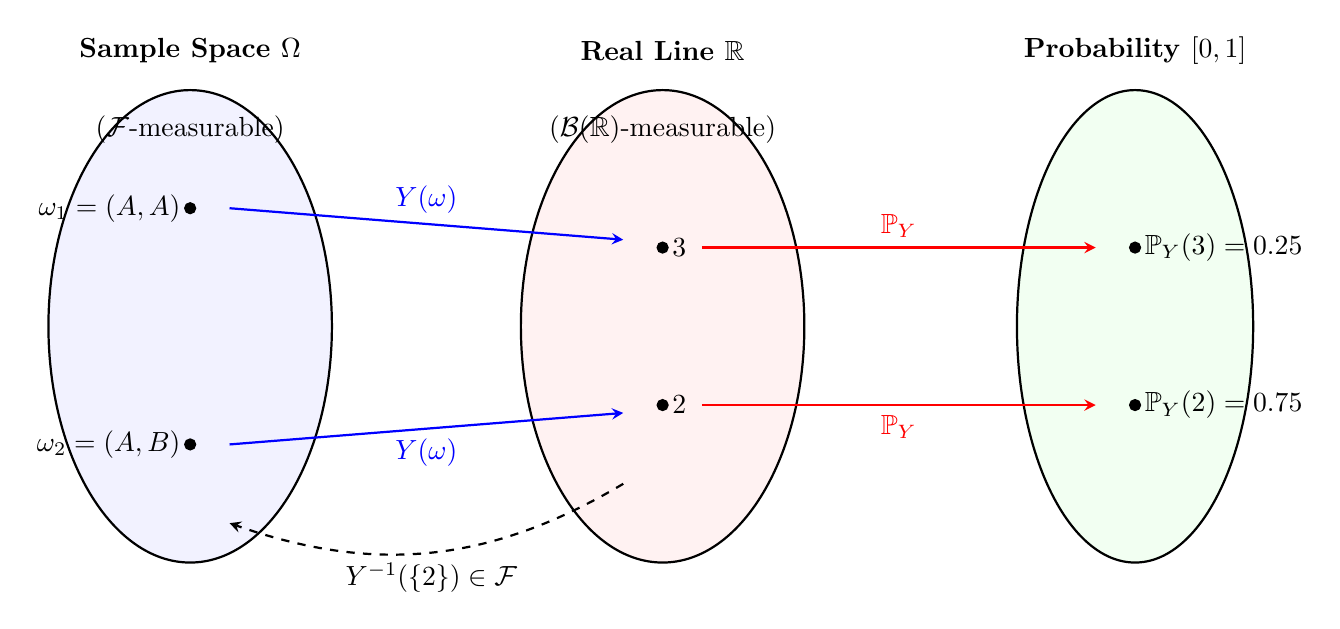
\begin{tikzpicture}[>=stealth]
    % Sample Space Omega
    \draw[thick, fill=blue!5] (0,0) ellipse (1.8cm and 3cm);
    \node at (0, 3.5) {\textbf{Sample Space $\Omega$}};
    \node at (0, 2.5) {$(\F\text{-measurable})$};
    
    % Real Line R
    \draw[thick, fill=red!5] (6,0) ellipse (1.8cm and 3cm);
    \node at (6, 3.5) {\textbf{Real Line $\R$}};
    \node at (6, 2.5) {$(\B(\R)\text{-measurable})$};
    
    % Probability Space [0,1]
    \draw[thick, fill=green!5] (12,0) ellipse (1.5cm and 3cm);
    \node at (12, 3.5) {\textbf{Probability $[0,1]$}};
    
    % Nodes
    \filldraw (0, 1.5) circle (2pt) node[left] {$\omega_1 = (A,A)$};
    \filldraw (0, -1.5) circle (2pt) node[left] {$\omega_2 = (A,B)$};
    
    \filldraw (6, 1) circle (2pt) node[right] {$3$};
    \filldraw (6, -1) circle (2pt) node[right] {$2$};
    
    \filldraw (12, 1) circle (2pt) node[right] {$\P_Y(3) = 0.25$};
    \filldraw (12, -1) circle (2pt) node[right] {$\P_Y(2) = 0.75$};
    
    % Function mappings Y
    \draw[->, thick, blue] (0.5, 1.5) -- (5.5, 1.1) node[midway, above] {$Y(\omega)$};
    \draw[->, thick, blue] (0.5, -1.5) -- (5.5, -1.1) node[midway, below] {$Y(\omega)$};
    
    % Induced Measure mapping P
    \draw[->, thick, red] (6.5, 1) -- (11.5, 1) node[midway, above] {$\P_Y$};
    \draw[->, thick, red] (6.5, -1) -- (11.5, -1) node[midway, below] {$\P_Y$};
    
    % Inverse image
    \draw[->, dashed, thick, black] (5.5, -2) to[bend left=25] node[midway, below] {$Y^{-1}(\{2\}) \in \F$} (0.5, -2.5);
\end{tikzpicture}
\end{center}

\subsection{Heuristics, Pitfalls, and Fallacies}
\begin{itemize}
    \item \textbf{Pitfall: The Base Rate Fallacy.} Occurs when interpreting conditional probabilities while ignoring the prior probability. Assuming $\P(B \mid A) \approx \P(A \mid B)$ is a fatal error. Always use Bayes' theorem to integrate the prior $\P(B)$.
    \item \textbf{Fallacy: Dividing by zero-probability events.} The conditional probability $\P(A \mid B) = \frac{\P(A \cap B)}{\P(B)}$ is strictly undefined if $\P(B) = 0$. Ensure $\P(B) > 0$ before proceeding.
    \item \textbf{Heuristic for Absorption.} Whenever a problem dictates ``repeat until $X$ occurs,'' you are invariably dealing with an infinite geometric progression. The probability of an event $A$ occurring before $B$ in independent sequences is strictly $\frac{\P(A)}{\P(A) + \P(B)}$.
\end{itemize}

% ==========================================
% PART 5: CONCEPTUAL SYNTHESIS
% ==========================================
\section{Conceptual Synthesis and The ``Big Picture''}

\subsection{Thematic Connections}
The ultimate theme of this section is \textbf{Measure-Theoretic Formalization of Randomness}. Earlier in statistics, one simply writes ``let $Y$ be the number of heads.'' Here, we synthesize this with rigorous set theory. $\Omega$ is a raw topological space. By passing the abstract events through a functional layer $Y$, we systematically ``pull back'' (via $Y^{-1}$) real-valued events into subsets of our $\sigma$-algebra $\F$, thereby inducing a structured probability measure on the real line. 

\subsection{Forward and Backward Links}
\textbf{Backward Link:} This concept relies heavily on axiomatic set theory and basic combinatorial arithmetic.
\textbf{Forward Link:} Constructing $Y$ as a measurable mapping is the absolute bedrock for defining the \textbf{Lebesgue Integral}, representing the Expected Value. Without ensuring $Y$ maps to Borel sets $\B(\R)$, we could not evaluate $\E[Y] = \int_{\Omega} Y(\omega) d\P(\omega)$. This exact integration technique expands into continuous-time Stochastic Calculus.

% ==========================================
% PART 6: ABSTRACT REAL-WORLD MODELING
% ==========================================
\section{Abstract Real-World Modeling (AI, ML, \& Quant Finance)}

\subsection{Concrete Scenarios}
\begin{enumerate}
    \item \textbf{Quantitative Finance (Algorithmic Trading):} Modeling the random movement of stock prices requires treating sequences of prices as random variables adapted to a \textit{filtration} $\F_t$ (a growing sequence of $\sigma$-algebras representing accumulating information over time).
    \item \textbf{Generative AI (Variational Autoencoders - VAEs):} In neural networks, an encoder maps a complex input space $\Omega$ (images) not to a deterministic vector, but to a latent probability space via a random variable $Z \sim \mathcal{N}(\mu(x), \sigma(x))$. The rigorous mapping rules of probability spaces constrain the optimization of the KL-divergence loss function.
\end{enumerate}

\subsection{Model Problem Setup: Asset Pricing via Geometric Brownian Motion}
To rigorously model a financial derivative, we establish a continuous probability space $(\Omega, \F, \mathbb{P})$ where the filtration $\{\F_t\}_{t \ge 0}$ tracks market data. Let $W_t$ be a standard Brownian motion (a stochastic sequence of random variables mapping outcomes $\omega$ to continuous paths).

We define the asset price $S_t$ not as a single number, but as a random variable governed by the Stochastic Differential Equation (SDE):
\[ dS_t = \mu S_t dt + \sigma S_t dW_t \]
where $\mu \in \R$ is the drift and $\sigma > 0$ is the volatility. The exact analytical solution utilizes Ito's Lemma (the stochastic equivalent of the Taylor Series):
\[ S_T(\omega) = S_0 \exp\left( \left(\mu - \frac{\sigma^2}{2}\right)T + \sigma W_T(\omega) \right) \]
In derivative pricing, an option payoff is a measurable function $Y(\omega) = \max(S_T(\omega) - K, 0)$. Because $S_T$ is a random variable, the composition function $Y$ is heavily verified to be $\F_T$-measurable, allowing quantitative analysts to price the option precisely by computing the Lebesgue integral $\E^{\mathbb{Q}}[e^{-rT}Y]$.

% ==========================================
% PART 7: COMMON VARIATIONS & UNTESTED CONCEPTS
% ==========================================
\section{Common Variations and Untested Concepts}

The provided text focused on strictly discrete finite subsets and probability mass. A severe conceptual gap exists regarding the formal transition to \textbf{Cumulative Distribution Functions (CDFs)}.

\begin{theorem}[Properties of a CDF]
For any random variable $Y$, its Cumulative Distribution Function $F_Y(y) = \P(Y \le y)$ is a rigorous extension of the probability measure satisfying:
1. $\lim_{y \to -\infty} F_Y(y) = 0$ and $\lim_{y \to \infty} F_Y(y) = 1$.
2. $F_Y(y)$ is monotonically non-decreasing.
3. $F_Y(y)$ is right-continuous.
\end{theorem}

\begin{proof}[Example Proof: Right-Continuity of CDF]
Let $y \in \R$ and let $(y_n)$ be a strictly decreasing sequence such that $\lim_{n \to \infty} y_n = y$.
We must prove that $\lim_{n \to \infty} F_Y(y_n) = F_Y(y)$.
Define the sets $A_n = \{\omega \in \Omega \mid Y(\omega) \le y_n\}$. 
Since $y_{n+1} < y_n$, $A_{n+1} \subset A_n$, meaning the sequence of sets is decreasing.
The intersection of all these sets is exactly $A = \{\omega \in \Omega \mid Y(\omega) \le y\}$.
By the continuity of probability measure axiom (derived from countable additivity):
\[ \lim_{n \to \infty} \P(A_n) = \P\left( \bigcap_{n=1}^\infty A_n \right) = \P(A) \]
Therefore, $\lim_{n \to \infty} F_Y(y_n) = F_Y(y)$. $\blacksquare$
\end{proof}

% ==========================================
% PART 8: ADVANCED DIAGNOSTIC TESTING
% ==========================================
\section{Advanced Diagnostic Testing: ``Find the Flaw''}

Act as the grader. Read the following five proofs, spot the singular fatal mathematical or logical fallacy, explain why it violates the axioms of probability or set theory, and uncover the truth in the solution key below.

\subsection{Diagnostic Problems}
\textbf{Problem 1: The Disjoint Union Trap}\\
\textit{Setup:} We are given an abstract probability space where $\P(A) = 0.7$ and $\P(B) = 0.6$. \\
\textit{Flawed Solution:} By Kolmogorov's third axiom of probability, the probability of the union is $\P(A \cup B) = \P(A) + \P(B) = 0.7 + 0.6 = 1.3$.

\textbf{Problem 2: The Conditional Divide}\\
\textit{Setup:} Let $A, B \in \F$. We wish to prove that if $A$ is independent of $B$, then $\P(A \mid B) = \P(A)$.\\
\textit{Flawed Solution:} By definition of independence, $\P(A \cap B) = \P(A)\P(B)$. Using the definition of conditional probability, we write $\P(A \mid B) = \frac{\P(A \cap B)}{\P(B)}$. Substituting the independence definition, $\P(A \mid B) = \frac{\P(A)\P(B)}{\P(B)} = \P(A)$. Q.E.D.

\textbf{Problem 3: The Uncounted Sample Point}\\
\textit{Setup:} An experiment consists of flipping two biased coins where $\P(Heads) = 0.6$. Let $Y$ be the number of heads. What is $\P(Y = 1)$?\\
\textit{Flawed Solution:} If $Y = 1$, we must see one head and one tail. The probability of a head is $0.6$ and a tail is $0.4$. Since the flips are independent, the probability is $\P(Y = 1) = 0.6 \times 0.4 = 0.24$.

\textbf{Problem 4: Infinite Sequence Convergence Fallacy}\\
\textit{Setup:} Consider an infinite sequence of coin flips where $E_n$ is the event that the $n$-th flip is a Head. $\P(E_n) = 0.5$. \\
\textit{Flawed Solution:} To find the probability that we get at least one head across the infinite timeline, we use the union bound (Boole's Inequality): $\P(\bigcup_{n=1}^\infty E_n) = \sum_{n=1}^\infty \P(E_n) = \sum_{n=1}^\infty 0.5 = \infty$.

\textbf{Problem 5: The Measurability Fallacy}\\
\textit{Setup:} Let $\Omega = \{a, b, c\}$ with $\sigma$-algebra $\F = \{\emptyset, \Omega, \{a\}, \{b, c\}\}$. We define a real-valued mapping $X(\omega)$ such that $X(a) = 1, X(b) = 2, X(c) = 3$.\\
\textit{Flawed Solution:} Since $X$ is a well-defined mathematical function mapping every element in the sample space $\Omega$ to a single element in $\R$, $X$ is inherently a valid random variable on this space. 

\subsection{Solution Key (Resolutions)}
\begin{enumerate}
    \item \textbf{Error in 1:} Kolmogorov's third axiom applies strictly and \textit{only} to mutually exclusive (disjoint) sets. Because $\P(A) + \P(B) = 1.3 > 1$, $A$ and $B$ cannot be mutually exclusive (by Unitarity). The correct formula is $\P(A \cup B) = \P(A) + \P(B) - \P(A \cap B)$.
    \item \textbf{Error in 2:} The step dividing by $\P(B)$ is invalid without explicitly asserting the assumption that $\P(B) > 0$. If $\P(B) = 0$, conditional probability $\P(A \mid B)$ is mathematically undefined.
    \item \textbf{Error in 3:} The setup ignores the combinatorial combinations. $Y=1$ maps to the pre-image $\{HT, TH\}$. The flawed solution calculated $\P(\{HT\})$ but omitted $\{TH\}$. The correct answer is $(0.6 \times 0.4) + (0.4 \times 0.6) = 0.48$.
    \item \textbf{Error in 4:} The union bound yields an upper bound of $\infty$, which provides zero predictive value. The fatal logical error is equating probability to $\infty$, violating the axiom $\P \le 1$. The true probability is derived via the complement: $\P(\text{at least one head}) = 1 - \lim_{n\to\infty}(0.5)^n = 1$.
    \item \textbf{Error in 5:} Measurability check failed. A function is only a random variable if all pre-images exist in $\F$. Taking the Borel set $B = \{2\}$, the pre-image is $X^{-1}(\{2\}) = \{b\}$. But $\{b\} \notin \F$. Therefore, $X$ is \textbf{not} a random variable on the given $\sigma$-algebra.
\end{enumerate}

\end{document}